%   ------------------------------------------------------------------------
\FloatBarrier
\subsection{Uso no pós-processamento}
\label{s.pixelLab.edicao}


Um dos principais usos do PixelLab.AI neste projeto foi como ferramenta de pós-processamento, aplicando ajustes finos manuais nos resultados gerados por outras ferramentas de forma que o resultado final já podia ser diretamente aplicado no jogo. A forma de exportação, o editor embutido e o ambiente em pixel art foram funcionalidades que trouxeram eficiência para essa etapa de correções, que é justamente o que falta na maioria das outras ferramentas.

Nessa seção, abordaremos as edições feitas que geraram o resultado final.

Como comentado em seções anteriores, o sprite do personagem Pablo em side view gerado pela ferramenta Gemini Pro (Figura \ref{fig:pixelLabPabloGeminiProSide}) passou por uma correção, onde os tons de cores e o tamanho foram ajustados, comparando o sprite lado a lado com a imagem do mesmo personagem de frente como pode ser visto nas Figuras \ref{fig:pixelLabFixSideViewComparaAntes} e \ref{fig:pixelLabFixSideViewComparaDepois}. Esse processo é extremamente importante, pois durante o jogo, o sprite de um personagem deve ser realmente consistente com os outros sprites daquele personagem, uma vez que haverá transições entre cada uma dessas figuras. Se a consistência não se mantém, em vez de apenas demonstrar um movimento ou mudança de posição, é causado um estranhamento no jogador. Posteriormente, uma nova edição foi realizada para ajustar detalhes como a falta de cabelo na nuca e o formato da orelha. Esse processo é demonstrado na Figura \ref{fig:pixelLabFinalSideView}.

\begin{figure}[htbp]
    \centering
    \caption{\small Comparação do sprite original e sprite gerado pelo Gemini Pro antes da edição}
    \label{fig:pixelLabFixSideViewComparaAntes}
    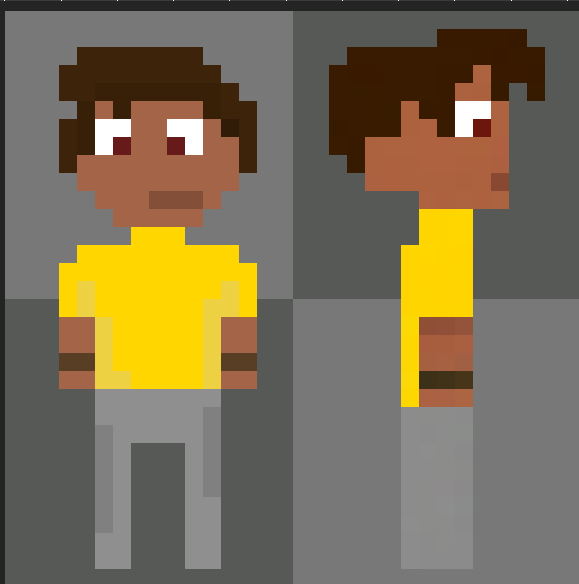
\includegraphics[width=0.4\linewidth]{figs/pixelLab/dia3/comparacao.PNG}
    \legend{\small Fonte: Elaborada pela autora.}
\end{figure}
    
\begin{figure}[htbp]
    \centering
    \caption{\small Comparação do sprite original e sprite gerado pelo Gemini Pro depois da edição}
    \label{fig:pixelLabFixSideViewComparaDepois}
    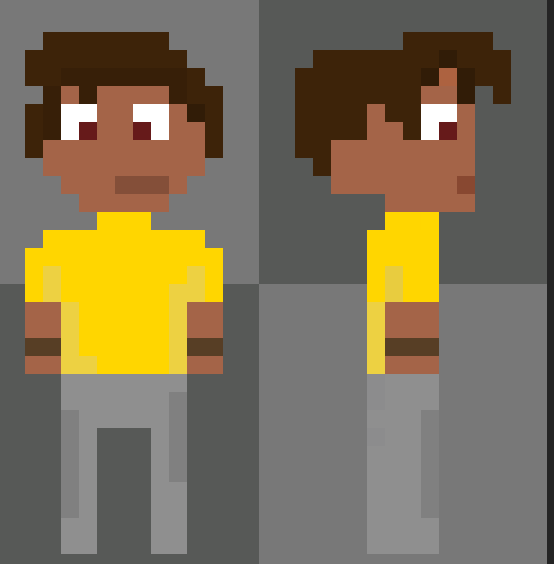
\includegraphics[width=0.4\linewidth]{figs/pixelLab/dia3/fix.PNG}
    \legend{\small Fonte: Elaborada pela autora, utilizando a ferramenta Pixel Lab.}
\end{figure}

\begin{figure}[htbp]
    \centering
    \caption{\small Processo de edição no Pixel Lab do sprite em side view gerado pelo Gemini Pro}
    \label{fig:pixelLabFinalSideView}
    \begin{subfigure}{0.32\linewidth}
        \centering
        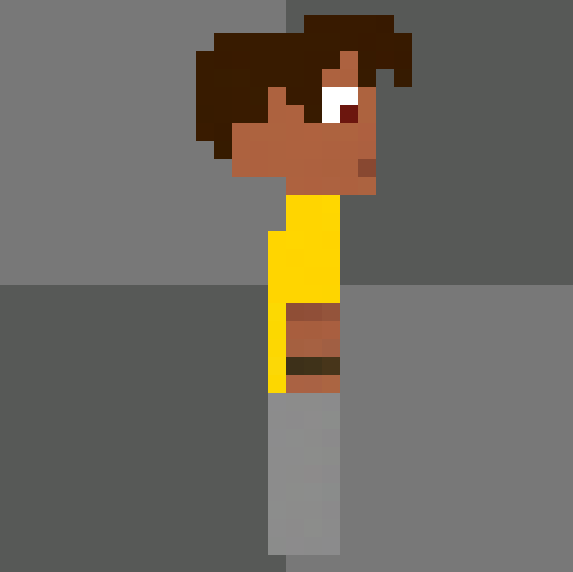
\includegraphics[width=1\linewidth]{figs/pixelLab/dia3/semFix.PNG}
        \caption{\small Antes da edição no Pixel Lab}
        \label{fig:pixelLabFinalSideView1}
    \end{subfigure}
    \begin{subfigure}{0.32\linewidth}
        \centering
        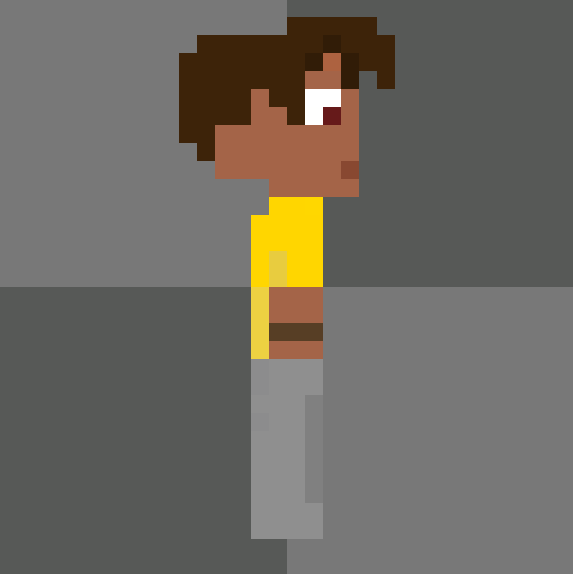
\includegraphics[width=1\linewidth]{figs/pixelLab/dia3/fixGrande.PNG}
        \caption{\small Após a primeira edição no Pixel Lab}
        \label{fig:pixelLabFinalSideView2}
    \end{subfigure}
    \begin{subfigure}{0.32\linewidth}
        \centering
        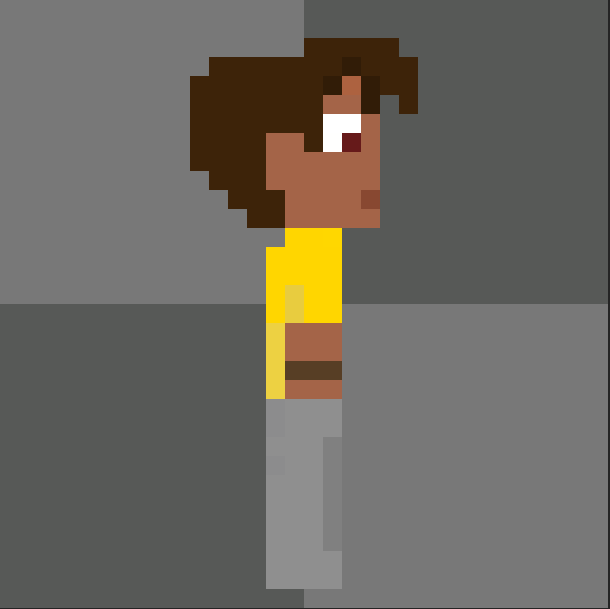
\includegraphics[width=1\linewidth]{figs/pixelLab/dia3/fix_oficial_fundo_igual.PNG}
        \caption{\small Resultado final}
        \label{fig:pixelLabFinalSideView3}
    \end{subfigure}

    \legend{\small Fonte: Elaborada pela autora, utilizando a ferramenta Pixel Lab.}
\end{figure}

Também foram realizados ajustes finos na, anteriormente apresentada, Figura \ref{fig:pixelLabPabloGeminiProCostas}, que mostra o sprite do personagem Pablo de costas gerado pelo Gemini Pro (detalhado na Seção \ref{s.ferramentaB}). O processo foi parecido com o do personagem em side view, usando a visão de frente para corrigir as cores e o tamanho da imagem. Além disso, pixels do que antes era o fundo branco foram apagados, mantendo a imagem com um fundo transparente. Esse processo pode ser verificado na Figura \ref{fig:pixelLabFinalBackView}.

\begin{figure}[htbp]
    \centering
    \caption{\small Processo de edição no Pixel Lab do sprite em back view gerado pelo Gemini Pro}
    \label{fig:pixelLabFinalBackView}
    \begin{subfigure}{0.45\linewidth}
        \centering
        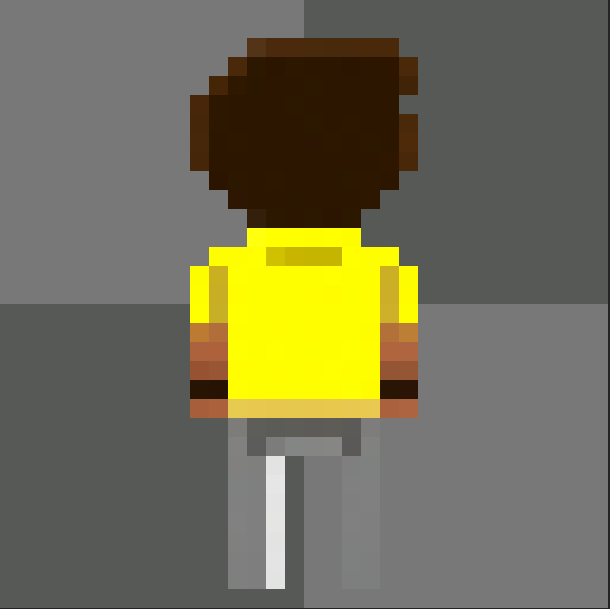
\includegraphics[width=1\linewidth]{figs/pixelLab/dia3/back_sem_fix.PNG}
        \caption{\small Antes da edição no Pixel Lab}
        \label{fig:pixelLabFinalBackView1}
    \end{subfigure}
    \begin{subfigure}{0.45\linewidth}
        \centering
        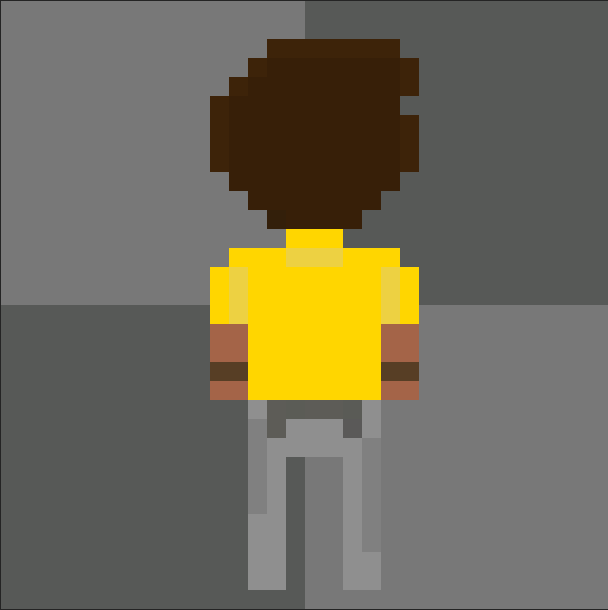
\includegraphics[width=1\linewidth]{figs/pixelLab/dia3/back_fix.PNG}
        \caption{\small Resultado final}
        \label{fig:pixelLabFinalBackView2}
    \end{subfigure}


    \legend{\small Fonte: Elaborada pela autora, utilizando a ferramenta Pixel Lab.}
\end{figure}

Os ajustes finos feitos no sprite sheet da porta abrindo em side view (Figura \ref{fig:pixelLabPortaViduSideView}) gerada pelo Vidu (detalhado na Seção \ref{s.vidu}) foram parcialmente parecidos com os anteriores, usando o sprite da porta fechada (Figura \ref{fig:pixelLabPortaSideView} para corrigir a altura, além de retirar qualquer pixel branco. Além disso, a moldura da porta (presente no sprite) foi fixada na mesma posição em todos os quadros, pois a moldura deve permanecer igual sem se mover mesmo quando a porta é aberta. Após isso, para cada um dos quadros, foi apagada a maçaneta ainda ligada à moldura, pintada novamente aquela parte da porta e desenhada uma nova maçaneta no canto correto. Após 12 quadros (dos 31 totais), foi observada que a porta praticamente não ficava mais aberta, com a maior parte dos outros frames igual ou muito similares. Dessa forma, os frames restantes foram apagados para não ocorrer perda de tempo em mudanças insignificantes.

A parte mais complexa do processo foi fazer novamente a maçaneta, pois era necessário entender o formato correto que ela ficaria dependendo do ângulo e como representar essa forma através dos tons de cores. Apesar disso, foi uma tarefa muito mais simples e rápida do que fazer a porta inteira do zero múltiplas vezes com cada frame tendo apenas pequenas modificações. O resultado desse processo final de edição pode ser verificado na Figura \ref{fig:pixelLabFinalPortaSideView}.

\begin{figure}[htbp]
    \centering
    \caption{\small Processo de edição no Pixel Lab do sprite sheet da porta gerado pelo Vidu}
    \label{fig:pixelLabFinalPortaSideView}
    \begin{subfigure}{0.45\linewidth}
        \centering
        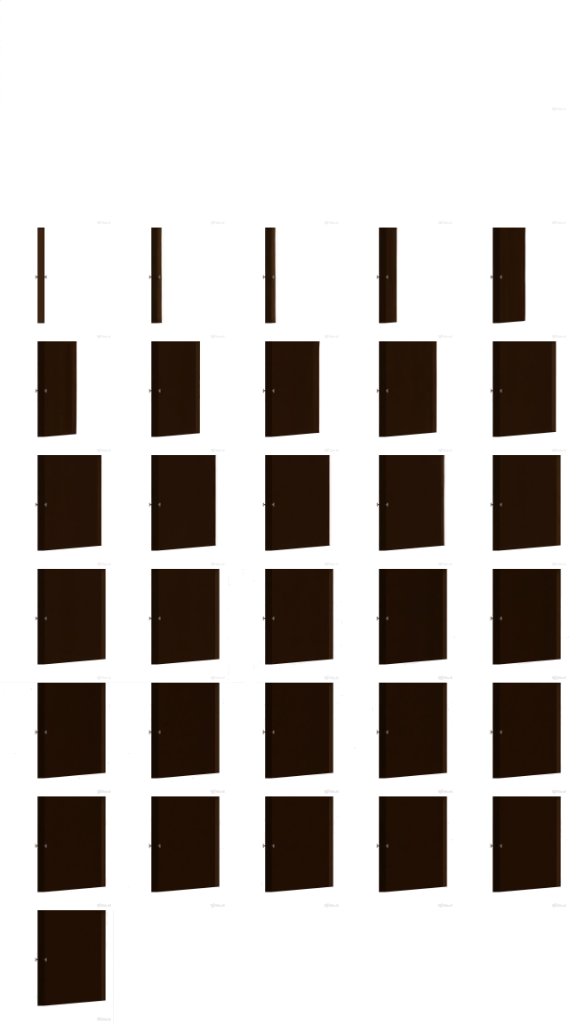
\includegraphics[width=1\linewidth]{figs/vidu/Pixilart/porta_sprite_sheet_pixel.png}
        \caption{\small Antes da edição no Pixel Lab}
        \label{fig:pixelLabFinalPortaSideView1}
    \end{subfigure}
    \begin{subfigure}{0.45\linewidth}
        \centering
        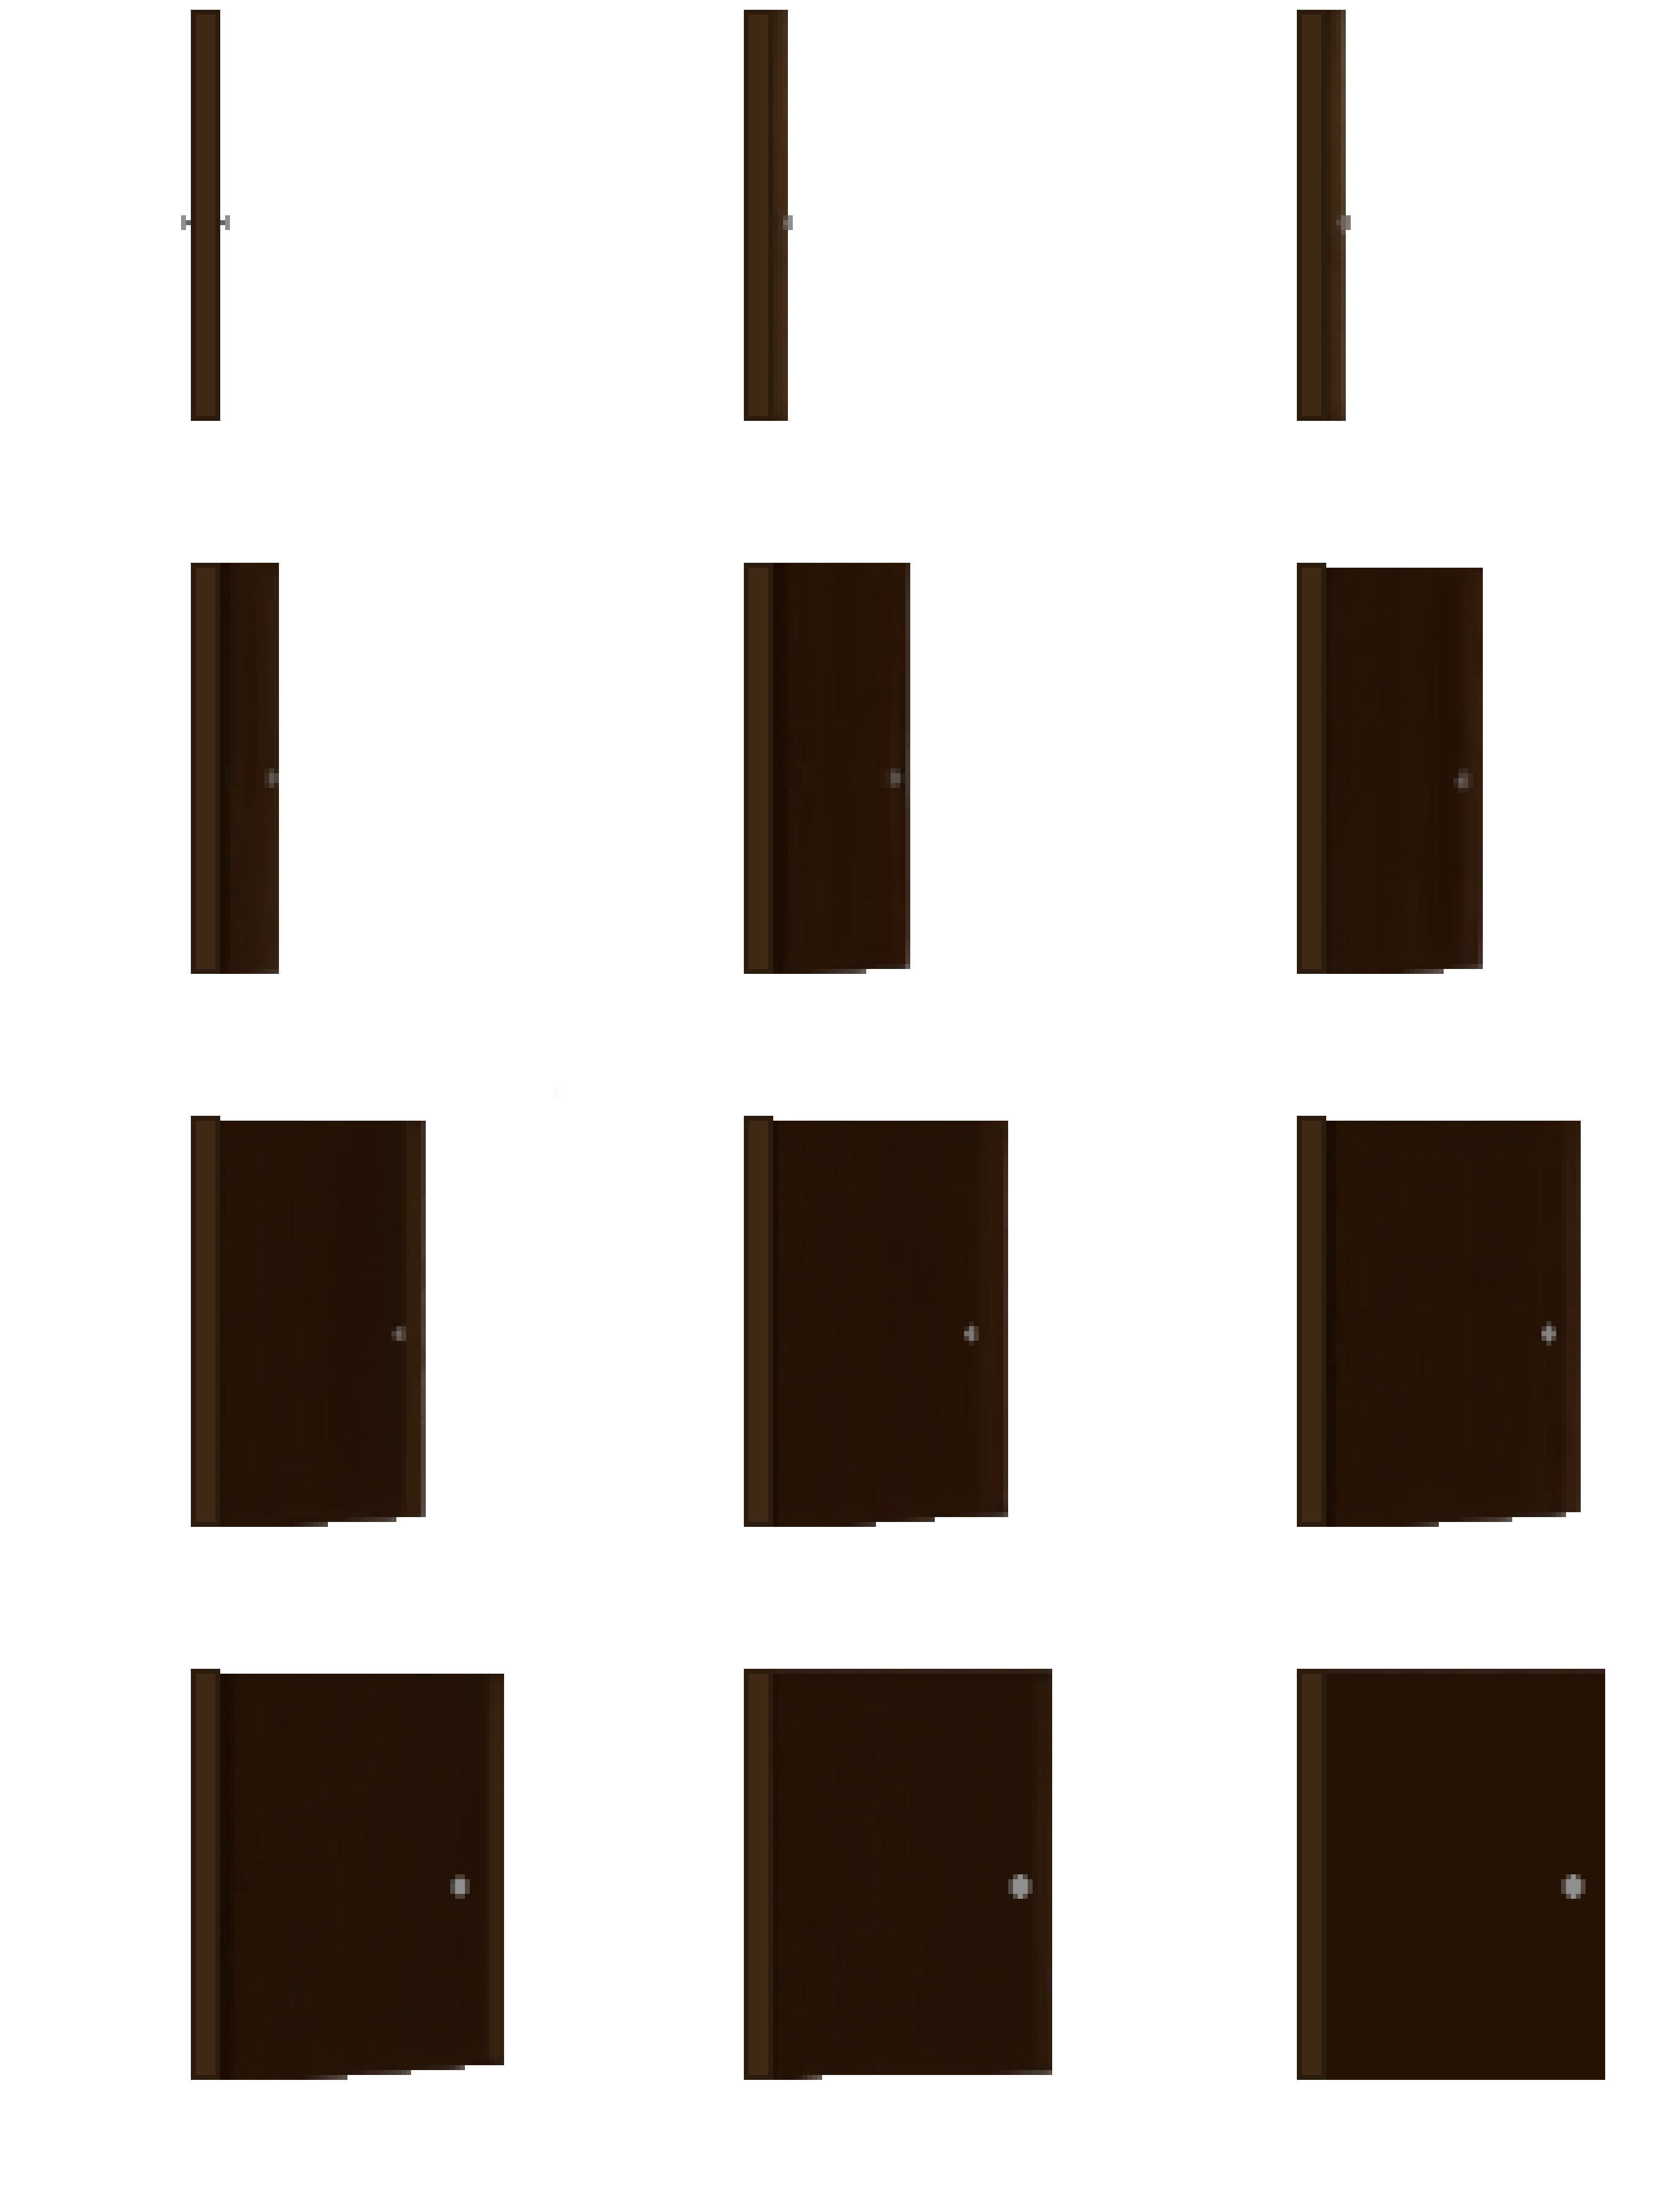
\includegraphics[width=1\linewidth]{figs/pixelLab/final/side_door_pixel_vidu.png}
        \caption{\small Resultado final}
        \label{fig:pixelLabFinalPortaSideView2}
    \end{subfigure}


    \legend{\small Fonte: Elaborada pela autora, utilizando a ferramenta Pixel Lab.}
\end{figure}